\documentclass[11pt,a4paper]{article}
\usepackage[margin=20mm]{geometry}
\usepackage{graphicx}
\usepackage{booktabs}
\usepackage{array}
\usepackage{xcolor}
\usepackage{colortbl}
\usepackage{enumitem}
\usepackage{fancyhdr}
\usepackage{titlesec}
\usepackage{hyperref}
\usepackage{float}
\usepackage{eurosym}

% Colors
\definecolor{danger}{RGB}{180,30,30}
\definecolor{warning}{RGB}{200,120,0}
\definecolor{safe}{RGB}{30,120,30}
\definecolor{headerblue}{RGB}{30,60,110}
\definecolor{lightgray}{RGB}{240,240,240}
\definecolor{rowalt}{RGB}{248,248,248}

% Header/footer
\pagestyle{fancy}
\fancyhf{}
\fancyhead[L]{\small\textbf{Kompic Mk1 PCB iv7.2 — Reflow \& Assembly Reference}}
\fancyhead[R]{}
\fancyfoot[C]{\thepage}
\renewcommand{\headrulewidth}{0.4pt}

% Section styling
\titleformat{\section}{\Large\bfseries\color{headerblue}}{}{0em}{}[\vspace{-0.5em}\rule{\textwidth}{0.4pt}]
\titleformat{\subsection}{\large\bfseries}{}{0em}{}
\titleformat{\subsubsection}{\normalsize\bfseries}{}{0em}{}

% Danger/warning boxes
\newcommand{\dangerbox}[1]{\par\noindent\colorbox{danger!10}{\parbox{\dimexpr\textwidth-2\fboxsep}{%
\textcolor{danger}{\textbf{WARNING:}} #1}}\par\vspace{0.5em}}

\newcommand{\notebox}[1]{\par\noindent\colorbox{headerblue!8}{\parbox{\dimexpr\textwidth-2\fboxsep}{%
\textcolor{headerblue}{\textbf{NOTE:}} #1}}\par\vspace{0.5em}}

\setlength{\parindent}{0pt}
\setlength{\parskip}{0.4em}

\begin{document}

% ============================================================
% TITLE
% ============================================================
\begin{center}
{\LARGE\bfseries\color{headerblue} Kompic Mk1 PCB — Reflow \& Assembly Reference}\\[0.3em]
{\large by Ivan Porupski, 2026}
\end{center}

% ============================================================
% PAGE 1 — QUICK REFERENCE
% ============================================================
\section*{PAGE 1 — QUICK REFERENCE {\small(keep visible during reflow)}}

\subsection*{Step-by-Step Procedure}

\begin{enumerate}[nosep]
\item Verify baked paste on all pads; smear thin flux (NC-559-ASM) across pad areas — flux QFN/WSON center pads too. For the MEMS mic, flux pads \textbf{before} placing, keep flux out of the top port.
\item Place all ICs and connectors onto flux + baked paste (tweezers, magnification). \textbf{All parts go on now — single reflow pass.}
\item Photograph the populated board; \textbf{attach thermocouple} to board edge with kapton tape.
\item Place board on \textbf{cold} hot plate, run the profile below. Hands off once heating starts; let the cycle finish before handling.
\end{enumerate}

\subsubsection*{Reflow Profile}

\begin{figure}[H]
\centering
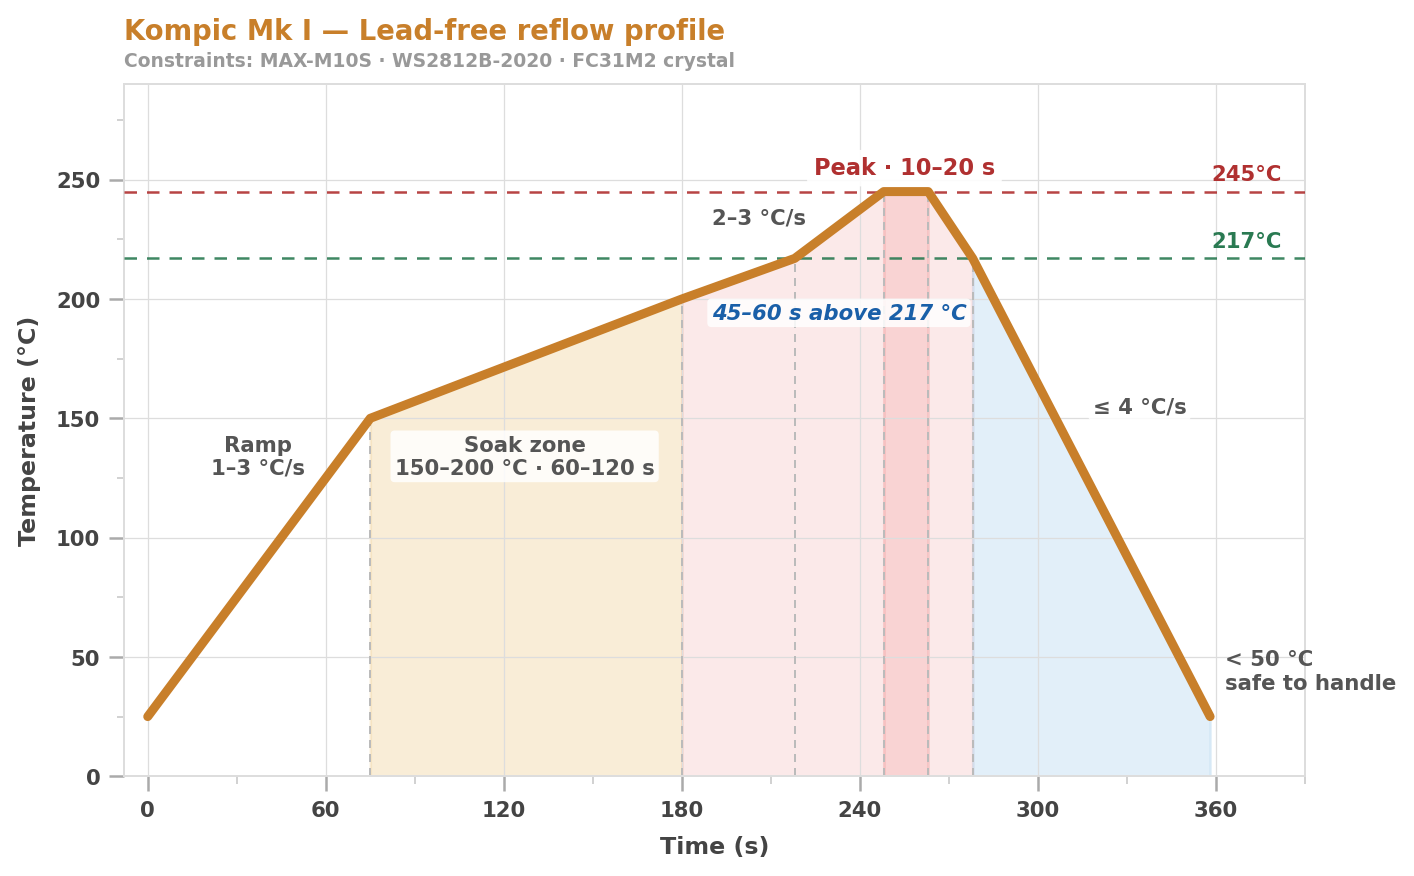
\includegraphics[width=0.95\textwidth]{reflow_profile.png}
\caption{\small Target reflow profile — binding constraints from MAX-M10S, WS2812B-2020, FC31M2 crystal.}
\end{figure}

\vspace{-0.5em}
\begin{table}[H]
\centering
\begin{tabular}{@{}ll@{}}
\toprule
\textbf{Phase} & \textbf{Target} \\
\midrule
Ramp to preheat & 1--3°C/s, 60--90s to reach 150°C \\
Soak & 150--200°C hold, 60--120s \\
Ramp to peak & 2--3°C/s \\
\rowcolor{danger!10} \textbf{Peak} & \textbf{245°C, hold 10--20s} \\
\rowcolor{danger!10} \textbf{Above 217°C total} & \textbf{45--60s} \\
Cooling & $\leq$ 4°C/s, hot plate off, natural cool \\
Safe to handle & Below 50--60°C \\
\bottomrule
\end{tabular}
\end{table}

\clearpage

\subsubsection*{During Heating — Rules}
\begin{itemize}[nosep]
\item \textbf{Hands off once heating starts.} No tapping, no nudging, no adjusting.
\item Below 217°C: if a part visibly shifts, you may carefully reposition with tweezers. This is a rescue, not routine.
\item Above 217°C (solder liquid): \textbf{\textcolor{danger}{DO NOT TOUCH ANYTHING.}} Surface tension self-centers parts.
\item If board gets bumped above 180°C: \textbf{let the cycle finish.} Never pull board off hot plate. Fix damage after cool-down.
\item Operate hot plate buttons with stable grip, controlled press, steady hand.
\end{itemize}

\subsubsection*{After Cooling}
\begin{enumerate}[nosep]
\item Visual inspection under magnification — every IC, every QFN edge, every pad
\item Compare against pre-reflow photo — check for shifted/rotated parts
\item Multimeter: resistance on every power rail to GND (3.2V, 1.8V, 5V, SYS, VBUS)
\item If all clear $\rightarrow$ initial power-on (see Page 2)
\item If short found $\rightarrow$ find and fix bridge before applying any power
\end{enumerate}

\subsection*{Floor Life — Bag Opening (all parts, single reflow)}

All MSL parts are placed in one pass, so open all moisture-sensitive bags on reflow day and reflow within their floor-life windows. Bake any part whose window was exceeded before placing.

\begin{table}[H]
\centering
\begin{tabular}{@{}llll@{}}
\toprule
\textbf{Part} & \textbf{MSL} & \textbf{Floor Life} & \textbf{Bake Recovery} \\
\midrule
ESP32-S3-WROOM-1U & 3 & $\sim$1 week at $<$30°C, $<$60\% RH & 125°C / 24hr \\
\rowcolor{danger!10} MAX-M10S & \textbf{4} & 72hr at $<$30°C, $<$60\% RH & 192hr @ 40°C, RH $<$5\% \\
\rowcolor{danger!10} VEML6030 & \textbf{4} & 72hr at $<$30°C, $<$60\% RH & 192hr @ 40°C, RH $<$5\% \\
\bottomrule
\end{tabular}
\end{table}

\dangerbox{Single reflow pass only. The board carries bottom-side components (notably the USB-C connector) that prevent a clean second hot-plate cycle — there is no second pass for any part. Every IC, including the MAX-M10S, must be placed and reflowed together. Plan placement so nothing is missed.}

% ============================================================
% PAGE 2 — BRING-UP SEQUENCE
% ============================================================
\newpage
\section*{PAGE 2 — BRING-UP SEQUENCE}

\subsection*{Initial Power-On}

\textbf{Current-limited LiPo test:}
\begin{itemize}[nosep]
\item 4$\times$ 200$\Omega$ 250mW resistors in parallel (= 50$\Omega$, 1W) in series with LiPo positive
\item Dead short draws 74mA max — nothing smokes
\item Measure voltage across board: $\sim$3.7V = no short, $\sim$0V = short present
\item ESP32 will NOT boot through this resistor (needs 300mA+) — this is shorts-only testing
\item Remove resistors for actual boot testing
\end{itemize}

\textbf{With USB power meter arrives:}
\begin{itemize}[nosep]
\item Power via USB-C through meter
\item Watch current draw in real time
\item BQ25619 boots first, brings up SYS rail, TPS62840 produces 3.2V
\item Normal idle current (no firmware): expect tens of mA
\item Stage-2 board (charger + RTC + bus 1 sensors + mic + WS2812 + USB-C, no display / GPS / daughter): \textbf{$\sim$100--120 mA} observed on USB-C with the stage-2 smoke sketch running (ESP32 active, sensors initialised, flashlight breathe loop). Use as ballpark, not a hard pass/fail.
\item If current spikes to 1A+ immediately: unplug, find the short
\end{itemize}

\notebox{The TPS62840 is VSET-programmable. A 3.3V rail is possible; this board deliberately uses a \textbf{3.2V} rail, set by a \textbf{100k} VSET resistor (instead of 172k for 3.3V). All 3.3V-domain parts remain within spec at 3.2V.}

\subsection*{Verification Sequence}

\begin{enumerate}[nosep]
\item Check 3.2V rail with multimeter — TPS62840 working?
\item Check 1.8V rail — XC6206 working?
\item Connect USB-C, check if ESP32 enumerates as USB CDC device
\item If ESP32 alive $\rightarrow$ I2C bus scan on bus 1 and bus 2
\item Every device should respond at expected address:
\end{enumerate}

\textbf{Bus 1:} 0x10 (VEML6030), 0x1C (LIS3MDLTR), 0x48 (TMP117), 0x51 (PCF85063), 0x57 (MAX30101), 0x5A (CST9217), 0x6B (LSM6DSV16X), 0x76 (BME688)

\textbf{Bus 2:} 0x5A (DRV2605), 0x6A (BQ25619)

\notebox{The MAX-M10S GPS is \textbf{not on I2C} by default — it communicates over \textbf{UART1} (GPS-TX $\rightarrow$ GPIO17, GPS-RX $\rightarrow$ GPIO18). Verify it by opening the UART and confirming NMEA/UBX traffic, not via an I2C scan. (The M10S DDC/I2C interface at 0x42 exists as an option but is unused on this board.)}

\begin{enumerate}[nosep,start=6]
\item Missing I2C device = suspect bad solder joint on that IC
\item Open UART1 (GPIO17/18) and confirm the M10S streams NMEA/UBX — GPS solder-joint check
\item Test 5V boost (BQ25619 PMID) — enable via I2C, confirm 5V on rail
\end{enumerate}

% ============================================================
% PAGE 3 — HIDDEN PAD IC VERIFICATION
% ============================================================
\newpage
\section*{PAGE 3 — HIDDEN PAD IC VERIFICATION}

These ICs have pads entirely underneath — you cannot visually inspect joints.

\begin{table}[H]
\centering
\renewcommand{\arraystretch}{1.3}
\begin{tabular}{@{}p{3.2cm}p{3cm}p{8cm}@{}}
\toprule
\textbf{Part} & \textbf{Package} & \textbf{Verification Method} \\
\midrule
BQ25619 & WQFN-24 (4$\times$4mm) & Highest risk. Check I2C response @ 0x6A. Measure SYS rail voltage. Check for bridges between perimeter pads and center GND. \\
MAX-M10S & LCC-18 & Castellated + bottom pads. Verify by opening UART1 (GPIO17/18) and confirming NMEA/UBX output. No second reflow available — get it right first pass. \\
BME688 & LGA-8 & I2C response @ 0x76. Read chip ID register. \\
LSM6DSV16X & LGA-14 & I2C response @ 0x6B. Read WHO\_AM\_I register. \\
LIS3MDLTR & LGA-12 & I2C response @ 0x1C. Read WHO\_AM\_I register. \\
MSM261DGT003 & MEMS mic & No I2C — test by reading PDM data. Clock on GPIO47, data on GPIO48. \\
TMP117 & WDFN-6-EP (2$\times$2mm) & I2C response @ 0x48. Read temperature register ($\sim$room temp). \\
PCF85063ATL & DFN-10 & I2C response @ 0x51. Read seconds register (should increment). \\
\bottomrule
\end{tabular}
\end{table}

\dangerbox{For all hidden-pad ICs: before reflow, don't add extra paste on top of JLCPCB stencil paste. Just flux. Excess paste under QFN/LGA causes bridges.}

% ============================================================
% PAGE 4 — SOLDER & CONSUMABLES
% ============================================================
\newpage
\section*{PAGE 4 — SOLDER \& CONSUMABLES}

\subsection*{What's On The Board}

JLCPCB assembles 0402 passives using SAC305 lead-free paste at 255$\pm$5°C (economic assembly). No passive has a peak temp limit below 260°C — no concern.

JLCPCB also applies SAC305 solder paste to ALL remaining pads via stencil (verify in their gerber viewer that paste layer apertures exist for IC pads). Paste is baked (not reflowed) before shipping. Builder reflows these pads on the hot plate at 245°C in a single pass.

Solder jumpers are pre-connected with cuttable traces — no soldering needed during assembly. Cut trace to change default state.

\subsection*{Your Consumables}

\begin{table}[H]
\centering
\renewcommand{\arraystretch}{1.3}
\begin{tabular}{@{}p{3.5cm}p{3.5cm}p{1.8cm}p{5.5cm}@{}}
\toprule
\textbf{Item} & \textbf{Alloy} & \textbf{Melting} & \textbf{Use On This Board} \\
\midrule
NC-559-ASM flux & — & — & \textcolor{safe}{\textbf{YES}} — apply to baked paste, rework \\
Sn99.3/Cu0.7 wire 0.8mm & Lead-free & 227°C & \textcolor{safe}{\textbf{YES}} — hand solder, rework, bridges \\
SAC305 syringe paste & Sn96.5/Ag3.0/Cu0.5 & 217°C & \textcolor{safe}{\textbf{YES}} — backup paste, rework touch-up \\
Sn62.8/Pb36.8/Ag0.4 paste & \textcolor{danger}{\textbf{LEADED}} & 181°C & \textcolor{danger}{\textbf{DO NOT USE ON THIS BOARD}} \\
\bottomrule
\end{tabular}
\end{table}

\dangerbox{The board arrives with SAC305 (lead-free) paste from JLCPCB. Mixing leaded paste with lead-free creates a mixed alloy with unpredictable melting point (181--217°C range). Joints form weak grain boundaries and fail as intermittent connections. \textbf{Keep all solder on this board lead-free.}}

\notebox{Sn99.3/Cu0.7 wire and SAC305 paste are not identical alloys (wire has no silver, paste has 3\% silver). This is fine — the small composition difference is negligible during rework. Both are lead-free, both melt in the 217--227°C range.}

\notebox{\textbf{Dire-straits fallback (prototype only, observed on Mk I iv7.1):} when lead-free SAC305 syringe paste cannot be obtained in time (this build waited 50+ days for delivery), a 50:50 mix of KEK flux + leaded paste (Sn62.8/Pb36.8/Ag0.4) applied \emph{only} to hidden center pads (QFN/LGA/DFN EP) reflows acceptably under the standard 245°C profile. Mixed-alloy boundaries form at those joints, against the absolute warning above --- on this first board every joint held through up to $\sim$6 rework cycles. This is a \textbf{prototype-only} workaround; long-term thermal-fatigue characteristics are unknown. The dangerbox stands as the production rule. Treat this note as the "if you must" caveat, not as permission.}

% ============================================================
% PAGE 5 — PRACTICE RUN
% ============================================================
\newpage
\section*{PAGE 5 — PRACTICE RUN \& TEMPERATURE CALIBRATION}

\subsection*{Before Your First Real Reflow}

\textbf{You must do at least one practice run.} Use a bare scrap board or one of your spare JLCPCB boards (no components).

\subsubsection*{Equipment Needed}
\begin{itemize}[nosep]
\item K-type thermocouple + reader ($\sim$\euro{}5--10) — \textbf{non-negotiable for 245°C ceiling with parts that die at 250°C}
\item Kapton tape to attach thermocouple to board surface
\end{itemize}

\subsubsection*{Procedure}
\begin{enumerate}[nosep]
\item Tape thermocouple tip flat against board surface, near center
\item Run your full reflow profile using hot plate buttons
\item Log thermocouple reading at each phase vs hot plate display reading
\item Calculate offset (e.g., hot plate says 245°C but board surface is actually 252°C $\rightarrow$ set hot plate to 238°C)
\item Run again with corrected settings, verify board surface hits 245°C $\pm$3°C
\item Note your hot plate button settings for each phase — these are your calibrated numbers
\end{enumerate}

\subsubsection*{What You're Calibrating}
\begin{itemize}[nosep]
\item Hot plate display accuracy (could be $\pm$10--15°C off)
\item Ramp rates (how fast does your specific plate heat and cool)
\item Cooling behavior (does it cool faster or slower than 4°C/s naturally)
\item Your button-pressing rhythm for each phase transition
\end{itemize}

\dangerbox{Without this calibration, you are guessing. A hot plate that reads 10°C low means you're actually hitting 255°C when you think you're at 245°C — and your M10S and WS2812B are over spec. With no second reflow available, a botched first pass is expensive — calibrate first.}

% ============================================================
% PAGE 6 — DAUGHTER PCB
% ============================================================
\newpage
\section*{PAGE 6 — DAUGHTER PCB REFLOW}

The daughter PCB (small round board) ships attached to the main PCB but should be reflowed separately.

\subsection*{Components on Daughter PCB}
\begin{itemize}[nosep]
\item MAX30101EFD+T (OLGA-14, 3.3$\times$5.6mm) — face down, HR/SpO2
\item TMP117AIDRVR (WDFN-6-EP, 2$\times$2mm) — skin temperature
\item DRV2605LDGSR (VSSOP-10) — haptic driver
\item Associated 0402 passives (JLCPCB assembled)
\end{itemize}

\subsection*{Profile}
Same as main board: 245°C peak, 45--60s above 217°C, $\leq$4°C/s cooling.

\subsection*{Risk Level}
Lower than main board. No MSL 4 parts, no WS2812B, no crystal. All three ICs tolerate 260°C. The 245°C profile gives generous margin. This is a straightforward reflow.

\subsection*{Inter-Board Connection}
After both PCBs are individually verified working, connect with 12 silicone wires (hand soldered to pads on each board).

% ============================================================
% PAGE 7 — REWORK PROCEDURES
% ============================================================
\newpage
\section*{PAGE 7 — REWORK PROCEDURES}

\subsection*{Solder Bridges (most common issue)}

\textbf{Method:} Soldering iron + flux + solder wick
\begin{itemize}[nosep]
\item Apply flux to bridged area
\item Press wick onto bridge with iron tip
\item Wick absorbs excess solder
\item Localized — only the affected pins experience thermal stress
\item This is always the first thing to try
\end{itemize}

\subsection*{Misaligned / Shifted IC}

\textbf{If visible pads} (castellated, gull-wing): reflow individual pins with iron, nudge into alignment with tweezers while last pin is still molten.

\textbf{If hidden pads} (QFN, LGA): must remove entirely. Use hot air rework station (controlled temp, focused nozzle). Pre-heat board on hot plate to 150°C, then hot air at 300--350°C on the IC until it lifts. Clean pads with wick + flux. Re-paste with SAC305 syringe, place new part, reflow locally.

\dangerbox{\textbf{Exception: MAX-M10S} — u-blox prohibits hot air. If M10S must be removed: pre-heat board on hot plate to 150°C, then use iron to release each castellated pad individually. Slow and tedious but possible for an LCC-18. Clean, re-paste, reflow locally.}

\subsection*{Dead IC (confirmed bad after electrical test)}

Same removal procedure as misaligned. Replace with spare from your doubles order. Localized rework only.

\dangerbox{There is \textbf{no second full reflow} on this board — bottom-side components (USB-C and others) prevent a clean second hot-plate cycle. All rework is \textbf{localized} (iron or focused hot air on the single failed part), never a whole-board re-reflow. Keep whole-board thermal cycles to the single production pass.}

% ============================================================
% PAGE 8 — COMPLETE COMPONENT REFLOW SPECS
% ============================================================
\newpage
\section*{PAGE 8 — COMPLETE COMPONENT REFLOW SPECIFICATIONS}

\subsection*{Binding Constraints Summary}

\begin{table}[H]
\centering
\begin{tabular}{@{}lll@{}}
\toprule
\textbf{Constraint} & \textbf{Value} & \textbf{Set By} \\
\midrule
Peak temperature & 245°C & MAX-M10S, WS2812B-2020 \\
Time above 217°C & 45--60s & MAX-M10S $\cap$ WS2812B-2020 \\
Time at peak ($\geq$240°C) & 10--20s & FC31M2 crystal \\
Max cooling rate & 4°C/s & MAX-M10S \\
\bottomrule
\end{tabular}
\end{table}

\subsection*{Full Component Table}

{\small
\begin{table}[H]
\centering
\renewcommand{\arraystretch}{1.15}
\begin{tabular}{@{}clllll@{}}
\toprule
\textbf{\#} & \textbf{Part} & \textbf{Package} & \textbf{MSL} & \textbf{Peak} & \textbf{Key Constraints} \\
\midrule
\rowcolor{danger!8}
1 & MAX-M10S-00B & LCC-18 & \textbf{4} & \textbf{245°C} & No hot air. Single reflow. No cleaning. \\
\rowcolor{danger!8}
2 & VEML6030 & — & \textbf{4} & 260°C & 72hr floor life. Bake if exposed. \\
\rowcolor{warning!8}
3 & ESP32-S3-WROOM-1U & Module & \textbf{3} & 235--250°C & Single reflow. Bake if open $>$1wk. \\
\rowcolor{danger!8}
4 & WS2812B-2020 & 2$\times$2mm & — & \textbf{245°C} & J-STD-020C. \\
5 & FC31M2-32.768kHz & SMD3215 & — & 260°C & 10s at peak. Cooling $\leq$6°C/s. \\
6 & Johanson 2450AT18A100E & Chip ant. & — & 260°C & 3 reflow cycles max. \\
7 & LSM6DSV16X & LGA-14 & — & 235--255°C & J-STD-020 (ST TN0018). \\
8 & LIS3MDLTR & LGA-12 & — & J-STD & J-STD-020. \\
9 & PCF85063ATL & DFN-10 & — & 260°C & Standard NXP. \\
10 & BME688 & LGA-8 & \textbf{1} & 260°C & 50$\mu$m min solder standoff. \\
11 & MSM261DGT003 & MEMS & — & 260°C & 5 reflow cycles OK. \\
12 & MAX30101EFD+T & OLGA-14 & — & 260°C & Max temp only stated. \\
13 & BQ25619RTWR & WQFN-24 & — & 260°C* & Assumed, TI QFN. \\
14 & TMP117AIDRVR & WDFN-6-EP & — & 260°C* & Assumed, TI WDFN. \\
15 & DRV2605LDGSR & VSSOP-10 & — & 260°C* & Assumed, TI VSSOP. \\
16 & TPD2E001DRLR & SOT-553 & — & 260°C* & Assumed, TI SOT. \\
17 & BSS138W & SOT-323 & — & 260°C* & Assumed, standard MOSFET. \\
18 & USB-C JS16T & 16-pin & — & 260$\pm$5°C & 60s $>$217°C, 5s $>$250°C. \\
\bottomrule
\end{tabular}
\end{table}
}
{\footnotesize *Not stated in datasheet — standard package assumption.}

\subsection*{MSL Handling Reference}

\begin{table}[H]
\centering
\begin{tabular}{@{}lll@{}}
\toprule
\textbf{MSL} & \textbf{Floor Life} & \textbf{Bake Recovery} \\
\midrule
1 & Unlimited & None needed \\
3 & $\sim$168hr (1 week) at $<$30°C, $<$60\% RH & 125°C / 24hr \\
4 & Per bag label ($\sim$72hr) at $<$30°C, $<$60\% RH & 192hr @ 40°C, RH $<$5\% \\
\bottomrule
\end{tabular}
\end{table}

\vfill

\subsection*{Notes}
\begin{itemize}[nosep]
\item Single reflow pass — bottom-side components (USB-C, etc.) preclude a second whole-board cycle. All parts, including MAX-M10S, go on together.
\item MAX-M10S communicates over \textbf{UART1} (GPIO17 TX / GPIO18 RX), not I2C. DDC/I2C @ 0x42 is available but unused.
\item All 0402 passives assembled and reflowed by JLCPCB at 255$\pm$5°C — their process, no passives at risk.
\item JLCPCB applies SAC305 solder paste to all remaining pads via stencil. Paste baked before shipping.
\item Pre-soldered 0402s re-melt during builder's reflow — board must be level and flat.
\item All solder on this board must be \textbf{lead-free}. Do not use leaded paste or wire.
\item Paste: SAC305 (Sn96.5/Ag3.0/Cu0.5), no-clean. Rework wire: Sn99.3/Cu0.7, 0.8mm. Flux: NC-559-ASM no-clean.
\item Core rail is \textbf{3.2V} via TPS62840 with a 100k VSET resistor (3.3V available with 172k; 3.2V chosen).
\item Boards are \textbf{1.0mm 4-layer}.
\end{itemize}

\vfill
\begin{center}\footnotesize
Kompic Mk1 — Reflow \& Assembly Reference \\
Revision iv7.0 \\
Ivan Porupski, 2026
\end{center}

% ============================================================
% PAGE 9 — STAGED (PROTOTYPE) BUILD
% ============================================================
\newpage
\section*{PAGE 9 — STAGED BUILD (prototype workflow, alternative to single-pass)}

\notebox{The prescribed flow is still \textbf{single reflow pass} (Pages 1--8). This page documents the \emph{prototype} flow used on the very first board, where confidence in each subsystem was built incrementally. If you are reproducing this build from scratch and want to de-risk one ring at a time, follow these stages. Each stage has a matching smoke-test sketch under \texttt{firmware/test/}.}

\subsection*{Stage 1 — Core (hot plate reflow)}

Minimal population required to boot the ESP32 and confirm both I2C buses are healthy.

\textbf{On board this stage:}
\begin{itemize}[nosep]
\item ESP32-S3-WROOM-1U-N16R8
\item BQ25619RTWR charger (bus 2 @ 0x6A)
\item TPS62840 3.2 V buck (100k VSET)
\item XC6206 1.8 V LDO
\item Flashlight LED + FET driver (GPIO41) with external pull-down
\item User button (BQ\_QON $\leftrightarrow$ GPIO16)
\item PCF85063ATL RTC (bus 1 @ 0x51) + FC31M2-32.768 kHz crystal + load caps
\item All JLCPCB-assembled 0402 passives (top and bottom)
\end{itemize}

\textbf{Excluded for this stage:} USB-C connector (bottom side — keep clear so the board can still hot-plate cleanly), all bus-1 sensors, mic, WS2812, daughter PCB, display connector, GPS.

\textbf{Reflow:} Full hot-plate profile per Page 1 (245°C peak, 45--60 s above 217°C). Single pass on the hot plate is uncomplicated here because the bottom side is empty.

\textbf{Power:} No USB-C yet — apply external 5 V to VBUS pad through a current-limited bench supply, or directly to SYS for a bypass test. \dangerbox{Never inject 5 V on a powered USB-C pad after stage 2 — the absent ESD diode on a missing USB-C JS16T is fine here because the connector itself isn't yet present.}

\textbf{Verification sketch:} \texttt{firmware/test/1\_smoke\_test\_mk1\_reflow1/1\_smoke\_test\_mk1\_reflow1.ino}

\textbf{Pass criteria:} ESP32 enumerates as USB CDC over the programming header (or external USB-UART, since USB-C is not yet on the board); BQ25619 ACKs at 0x6A with sane STATUS/PART/FAULT; PCF85063A ACKs at 0x51 with OS bit clear (oscillator running); button toggles the flashlight; flashlight LEDC breathe visible.

\subsection*{Stage 2 — Sensing + USB-C (hot air, no more hot-plate cycles)}

\textbf{Added this stage:}
\begin{itemize}[nosep]
\item USB-C JS16T receptacle (bottom side) + TPD2E001 ESD
\item VEML6030 ambient light sensor (bus 1 @ 0x10)
\item LIS3MDLTR magnetometer (bus 1 @ 0x1C)
\item LSM6DSV16X IMU (bus 1 @ 0x6B)
\item BME688 environmental sensor (bus 1 @ 0x76)
\item MSM261DGT003 PDM microphone (I2S: CLK GPIO47, DATA GPIO48)
\item WS2812B-2020 signal LED (one-wire DIN @ GPIO42)
\end{itemize}

\textbf{Why hot air from here on:} the USB-C JS16T is bottom-side. Once it is placed, the board can no longer be put face-down on the hot plate without melting it; equally, face-up reflow risks reflowing the USB-C joints uncontrolled. \textbf{Stage 2 closes the hot-plate window for this board.} All further additions are localised hot-air or iron rework.

\textbf{Procedure:}
\begin{enumerate}[nosep]
\item Flux all stage-2 pads. For the MEMS mic, flux pads \emph{before} placing and keep flux out of the top port.
\item Place all stage-2 ICs and the USB-C connector. Bottom-side USB-C should be done last with the board flipped on a holder, hot air at 300--350°C, focused nozzle, generous flux. Watch the mic and the QFN/LGA islands on the top side for any heat that telegraphs through.
\item Reflow each top-side IC locally with focused hot air. Don't park hot air on the WS2812 — its 245°C ceiling is a tight box even at the IC scale.
\end{enumerate}

\textbf{Electrical pre-checks (before powering):}
\begin{itemize}[nosep]
\item Multimeter continuity / resistance: VBUS-to-GND, 3V3-to-GND, 1V8-to-GND $\rightarrow$ no shorts.
\item SDA/SCL (both buses) to GND $\rightarrow$ no shorts; bus 1 SDA $\leftrightarrow$ SCL not shorted; bus 2 SDA $\leftrightarrow$ SCL not shorted.
\item Plug into USB-C through an inline current meter (USB-C power meter, USB tester, or bench supply set to 5 V with current limit).
\item Expected steady-state draw: \textbf{$\sim$100--120 mA} with the stage-2 smoke sketch running. Above $\sim$300 mA at idle, or any visible smoke / smell, $\rightarrow$ unplug immediately and inspect.
\end{itemize}

\textbf{Verification sketch:} \texttt{firmware/test/2\_smoke\_test\_mk1\_hotair/2\_smoke\_test\_mk1\_hotair.ino}

\textbf{Pass criteria:} I2C scan returns the full expected stage-2 set --- \mbox{bus 1 = \{0x10, 0x1C, 0x51, 0x6B, 0x76\}} and \mbox{bus 2 = \{0x6A\}}; each chip's WHO\_AM\_I / chip-ID matches; WS2812 colour walk is visible; PDM mic returns non-zero samples; the 1 Hz round-robin loop continues to print live values from every device without dropouts. Missing addresses point at suspect solder joints on that specific chip.

\subsection*{Stage 3 — Daughter PCB + storage (hot air / iron)}

\textbf{Added this stage:}
\begin{itemize}[nosep]
\item Micro-SD card slot + associated routing
\item Daughter PCB (small round board), reflowed \emph{separately} on the hot plate per Page 6: MAX30101 (bus 1 @ 0x57), TMP117 (bus 1 @ 0x48), DRV2605 (bus 2 @ 0x5A)
\item 12 silicone wires hand-soldered between main PCB and daughter PCB
\end{itemize}

\textbf{Procedure:} reflow the daughter PCB on its own (full profile, no constraints from the main board), verify it standalone with a small bench fixture, then connect to the main board via the 12 inter-board wires. Hot-air or iron the SD card slot onto the main board.

\textbf{Pass criteria:} I2C scan now also shows 0x48, 0x57 on bus 1 and 0x5A on bus 2; SD card mounts and writes a test file; DRV2605 buzzes when triggered.

\subsection*{Stage 4 — Display + touch}

\textbf{Added this stage:}
\begin{itemize}[nosep]
\item CO5300 2.06" AMOLED + CST9217 capacitive touch on the 24-pin FPC
\item OK-14F024-04 receptacle (J1) mated to the display ribbon
\end{itemize}

\textbf{Procedure:} the receptacle is hand-soldered or hot-air'd to the main board. Display panel mates to the connector --- no reflow on the panel itself. CST9217 lives on the display assembly (bus 1 @ 0x5A), so it only joins the I2C scan once the panel is plugged in.

\textbf{Pass criteria:} CO5300 driver brings the panel up at COLMOD 0x77 (RGB888) via QSPI on the SPI2/FSPI IOMUX pins; CST9217 ACKs at 0x5A and reports touch events; panel survives a sleep cycle (DISPOFF 0x28 $\rightarrow$ SLPIN 0x10 $\rightarrow$ SLPOUT 0x11 + re-init $\rightarrow$ DISPON 0x29).

\subsection*{Stage 5 — GPS (MAX-M10S, deliberate last)}

\textbf{Added this stage:}
\begin{itemize}[nosep]
\item u-blox MAX-M10S-00B (LCC-18, MSL 4) --- soldered first
\item Johanson 2450AT18A100E (or equivalent) chip antenna --- soldered \emph{after} the M10S is on and verified
\end{itemize}

\textbf{Why last in this prototype flow:} the MAX-M10S has the tightest constraints on the board (245°C peak, no hot air, no cleaning, MSL 4). On the prescribed single-pass workflow it sits in the same reflow as everything else. In this staged workflow, the hot-plate window has been closed by stage 2 --- so the M10S goes on by hand, via the iron-on-castellation procedure from Page 7:

\begin{enumerate}[nosep]
\item Bake the M10S per its floor-life recovery (192 hr @ 40°C, RH $<$ 5\%) if its MSL window has been exceeded since opening the bag.
\item Pre-heat the main board on the hot plate to 150°C (well below all the stage-2 parts' reflow points, USB-C handles this fine).
\item Pre-tin each castellated pad on the M10S footprint with a tiny SAC305 solder bump using the iron + flux.
\item Place the M10S, then reflow each castellation locally with the iron + flux + Sn99.3/Cu0.7 wire. Slow and tedious but well within tolerance for an LCC-18 with exposed castellations.
\item No solvents, no clean --- M10S datasheet forbids cleaning.
\item \textbf{Verify the M10S electrically before placing the antenna:} open UART1 (GPIO17/18) at 9600 baud, confirm NMEA / UBX traffic, and check no shorts on the antenna pad. The antenna goes on \emph{after} the M10S is confirmed alive --- placing it earlier risks reworking the M10S with the chip antenna already in the heat zone (the Johanson chip antenna tolerates standard SMD reflow but should not see repeated rework cycles).
\item \textbf{Hand-solder the antenna last:} iron + flux + Sn99.3/Cu0.7 wire on the two antenna pads. Keep the iron contact $<$ 3 s per pad. After it is on, confirm the GPS still streams NMEA, then observe time-to-first-fix outdoors (cold-start can be several minutes).
\end{enumerate}

\dangerbox{This is the \emph{prototype} accommodation. The intended production workflow is the single-pass reflow on Pages 1--8, where MAX-M10S goes through the controlled hot-plate profile with everything else. Iron-on-castellations is a fallback and adds risk --- expect to use a spare M10S if the first attempt cooks an internal joint.}

\textbf{Pass criteria:} open UART1 (GPIO17 TX / GPIO18 RX) at 9600 baud and confirm NMEA / UBX traffic streaming from the M10S; 1PPS edge visible on GPIO46 once a fix is obtained.

\subsection*{Stage Summary}

{\small
\begin{table}[H]
\centering
\renewcommand{\arraystretch}{1.2}
\begin{tabular}{@{}cp{3.2cm}p{4.0cm}p{3.4cm}p{3.4cm}@{}}
\toprule
\textbf{Stage} & \textbf{Process} & \textbf{Adds} & \textbf{New I2C} & \textbf{Smoke sketch} \\
\midrule
1 & Hot plate (full profile)          & Core + RTC                                 & 0x51 (b1), 0x6A (b2)         & 1\_smoke\_test\_mk1\_reflow1 \\
2 & Hot air (closes hot-plate window) & USB-C + bus-1 sensors + mic + WS2812       & 0x10, 0x1C, 0x6B, 0x76 (b1)  & 2\_smoke\_test\_mk1\_hotair  \\
3 & Hot air / iron + separate reflow  & SD + daughter PCB                          & 0x48, 0x57 (b1), 0x5A (b2)   & --- (per-chip tests) \\
4 & Hand solder + mate                & Display panel + touch                      & 0x5A (b1)                    & --- (display driver) \\
5 & Iron on castellations             & MAX-M10S + antenna                         & --- (UART1, not I2C)         & --- (NMEA dump) \\
\bottomrule
\end{tabular}
\end{table}
}

\notebox{If you are reproducing the prototype flow: keep a written log of what current the board draws at each stage with each smoke sketch running. Drift in that idle figure stage-over-stage is the cheapest early warning of a marginal joint.}

\end{document}